\chapter{Introducción} \label{cap:introduccion}
%\section{Introducción} \label{s:introduccion}
\pagenumbering{arabic}
\setcounter{page}{1}
El presente TFM se encuadra dentro de la Visión Artificial y en particular en el campo de la Autolocalización Visual, que tiene numerosas aplicaciones entre las que destacan la robótica y la realidad aumentada.
Actualmente la investigación y desarrollo en robótica móvil está en pleno auge. Los robots modernos están equipados con múltiples sensores y uno de los más utilizados son las cámaras, ya que permiten al robot captar en imágenes todo el entorno que le rodea. En contra partida, el procesado de imágenes conlleva una carga notable de CPU debido a la enorme cantidad de información que puede aportar cada imagen.

Una de las funcionalidades más importantes que se persigue, es que los robots móviles puedan desplazarse por su entorno y navegar desde la posición A a la posición B de forma autónoma y para ello una habilidad fundamental es la Autolocalización. 
Esta tarea no resulta muy complicada en entornos estructurados, donde el robot conoce de antemano el terreno por el que se mueve o sabe de la existencia de alguna baliza que le dé pistas de su posición.
Pero en entornos no estructurados, donde el robot desconoce por completo el terreno, carece de mapas y no existe a priori ningún tipo de marca o baliza que pueda guiar al robot, la Autolocalización resulta mucho más compleja.


Visual SLAM (\textit{Simultaneous Localization and Mapping}) es una técnica utilizada principalmente con robots móviles equipados con cámaras y que aporta al robot la capacidad de autolocalizarse y generar mapas del entorno que le rodea en tiempo real gracias al procesamiento de imágenes. Gracias a ese mapa y principalmente a esa autolocalización se pueden utilizar las técnicas de navegación autónoma, que requieren inevitablemente de una estimación de posición propia fiable. 

El robot debe contar con una capacidad de cálculo suficiente que le permita ejecutar el software de procesado de imágenes y al mismo tiempo realizar la generación de mapas. Estas tareas requieren ser ejecutadas en tiempo real, unos 30 fotogramas por segundo. 



\section{Visión Artificial}
La Visión Artificial es una rama científico técnica creada para extraer y procesar información a partir de imágenes.

Sus inicios, se remontan hacia mediados del siglo pasado, cuando en 1961 Larry Roberts desarrolló en la universidad un programa que era capaz de ver una estructura de bloques, analizar su contenido y reproducirla desde otra perspectiva, para ello tuvo que utilizar los dos componentes principales de un sistema de visión artificial , una cámara y necesariamente un ordenador. Pero debido a la alta complejidad de las tareas de visión artificial y a la primitiva capacidad de proceso  de las computadoras de la época, los resultados en la investigación sobre visión artificial fueron muy limitados y podemos decir que la evolución de la visión artificial ha ido ligada a los avances en la computación. Con la aparición de microprocesadores más rápidos, el aumento exponencial de la memoria y la creación y mejora de los algoritmos  se han ido consiguiendo mejores resultados hasta crear sistemas de visión artificial que son capaces de operar en tiempo real, permitiendo que un automóvil sea capaz de conducir de forma autónoma, o que un robot sea capaz de agarrar una pelota cuando se la lanzamos.

\begin{figure}[htbp]
\begin{center}
%\subfigure[]{\label{fig:RobotShakey}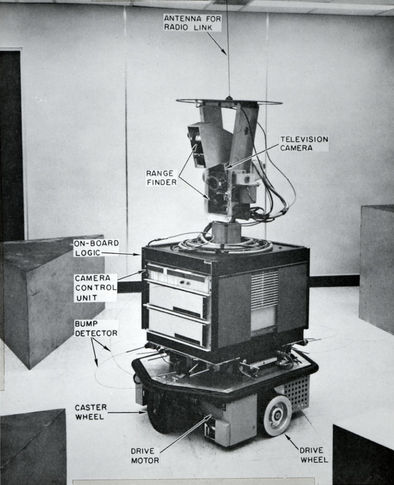
\includegraphics[height=8.0cm]{img/cap2/RobotShakey.jpg}}
\label{fig:RobotShakey}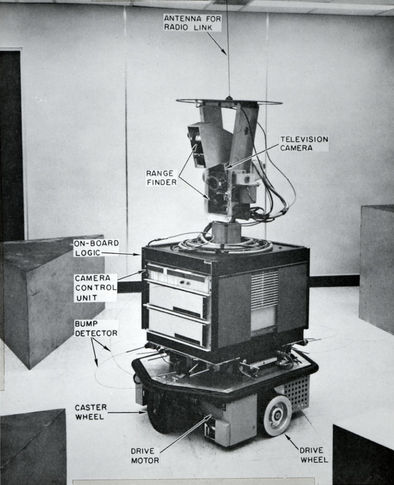
\includegraphics[height=8.0cm]{img/cap2/RobotShakey.jpg}
\end{center}
\caption{Robot Shakey. En los albores de la Visión Artificial}
\end{figure}


\subsection{Bloques habituales en sistemas de Visión Artificial}
La mayoría de sistemas de visión artificial o visión por computador están compuestos por dos elementos principales:  El sistema de adquisición de imágenes y el sistema de procesado de imágenes. El primero se compone de la iluminación, captura de imágenes y sistemas de adquisición de señales. El segundo implementa los algoritmos de visión que procesan las imágenes para extraer información de ellas.

	\textbf{- El sistema de iluminación}: Está compuesto por todos los elementos que iluminan los objetos con cualquier tipo de radiación electromagnética. Como ejemplo de estos artefactos podríamos citar la luz natural del sol, o la luz artificial proporcionada por lámparas, lasers o leds.

	\textbf{- El sistema de captura de imagen}: Transforma en señales eléctricas la luz que se refleja en los objetos. El elemento más utilizado son las cámaras, tanto de espectro visible como de espectro invisible.

	\textbf{- El sistema de adquisición de señales}: Las imágenes capturadas por las cámaras se utilizan para generar señales de vídeo. Su principal objetivo es enviar la señal de vídeo a la entrada de datos del ordenador.

	\textbf{- Sistema de procesamiento}: Suele ser un ordenador u otro dispositivo con capacidad de computación que implementa los algoritmos necesarios para procesar la imagen digital y para elaborar la información requerida por el sistema de visión artificial

	El sistema de procesamiento de imágenes suele componerse de las siguientes fases:
    \begin{enumerate}
		\item{Preproceso}: Durante esta fase la imagen puede ser adaptada para extraer mejor la información requerida por los algoritmos o métodos usados. El principal objetivo de esta fase es obtener una mejor calidad de la imagen de entrada, usando técnicas como filtrados de ruidos, convolución, resaltado de bordes etc.

		\item{Segmentación}: En esta fase la imagen es dividida en áreas de interés. Por ejemplo diferenciando objetos cuadrados de objetos esféricos o seleccionando las líneas de la carretera obviando el resto de la imagen. Para este propósito se pueden utilizar varias técnicas: umbrales, discontinuidades, crecimiento de regiones, filtros de color, detección de movimiento, etc

		\item{Clasificación}: Una vez la imagen ha sido dividida por regiones de interés (\textit{Regions of Interest}), se pueden extraer las características específicas de cada una. Esto puede realizarse por análisis morfológico , por texturas o usando técnicas de clasificación de color.
	\end{enumerate}

	\textbf{- Sistemas Periféricos}: Se trata de los elementos receptores de información, incluyendo monitores, dispositivos que usan la información par tomar decisiones etc.

\subsection{Aplicaciones de Visión Artificial}
Hoy en día, el número de aplicaciones de visión por computador está creciendo muy deprisa, debido a la disponibilidad de hardware barato que es capaz de ejecutar complejos algoritmos de visión artificial en un tiempo razonable. Por ejemplo, podemos encontrar aplicaciones en robótica para vehículos no tripulados, en medicina la visión artificial ya ayuda en diagnósticos mediante análisis de imágenes de los pacientes ( cáncer, enfermedades degenerativas, etc), en astronomía ayuda a generar imágenes de mayor calidad etc.

Actualmente, la visión artificial se utiliza en muchos procesos científicos, industriales y militares, por ejemplo para el reconocimiento de objetos o en el seguimiento de éstos:

	\textbf{Reconocimiento de objetos}: Se trata de buscar unas propiedades concretas de un determinado objeto (forma, color o cualquier otro patrón) en una imagen para determinar si un objeto se encuentra o no en ella. Por ejemplo mediante la obtención de píxeles característicos que destaquen en la imagen o utilizándose técnicas de \textit{Deep Learning} con redes neuronales.

	\textbf{Seguimiento de objetos}: Tras ser detectado, se pueden realizar tareas de seguimiento de un objeto. Podrá efectuarse dicho seguimiento teniendo en cuenta sus propiedades (texturas, bordes, etc) o analizando su desplazamiento respecto a imágenes anteriores.

	\textbf{Reconocimiento de caracteres (OCR)}:  Una de las aplicaciones más populares para la visión artificial es el reconocimiento de caracteres (OCR). El propósito de estos sistemas son la identificación de caracteres, por ejemplo hay aplicaciones que te permiten sacar una foto a la lista de componentes de un producto envasado y la aplicación gracias al OCR puede revisar todos los ingredientes del alimento y avisar si el producto contiene algún elemento al que pueda ser alérgico el usuario, como por ejemplo el gluten.

	\textbf{Aplicaciones de realidad aumentada}: gracias a la Visión Artificial es posible capturar imágenes del mundo real y procesarlas añadiendo la posibilidad de introducir en estas imágenes elementos artificiales nuevos (gráficos 3D) que encajarían en las dimensiones de las imágenes capturadas. Por ejemplo podríamos captar imágenes de una habitación de la casa a través de la cámara del móvil y mediante realidad aumentada añadir mobiliario nuevo virtual que sólo sería observable desde la pantalla del smartphone.

\begin{figure}[htbp]
\begin{center}
\label{fig:realiadAumentada}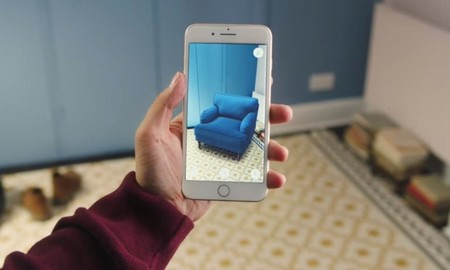
\includegraphics[height=8.0cm]{img/cap2/realidadAumentada.jpg}
\end{center}
\caption{Ejemplo de realidad aumentada, el sillón sólo existe en la pantalla del smartphone}
\end{figure}


\section{Visual SLAM}

\textit{Visual Simultaneous Localization And Mapping} (Localización y Mapeo Visual Simultaneo). Se refiere al proceso de estimar la posición y orientación de una cámara con respecto al mundo que le rodea, mientras que simultáneamente mapea el espacio que rodea a la cámara gracias a un procedimiento que analiza y extrae información de las imágenes capturadas por dicha cámara.

Visual SLAM es un tipo específico de sistema SLAM que se basa en algoritmos de visión 3D
para realizar tareas de autolocalización y mapeo cuando ni la localización de la posición de la cámara ni el entorno son conocidos.

La mayoría de los sistemas SLAM funcionan estimando la posición de un conjunto de puntos en varias imágenes sucesivas y así triangular la posición 3D, mientras que simultáneamente utiliza esta información para dar un posición aproximada de la cámara. Básicamente, el objetivo de estos sistemas es hacer un mapa de sus alrededores de su localización para así poder realizar tareas de navegación por el entorno.

Esto es posible con una sola cámara. Mientras existan un número suficiente de puntos que puedan ser seguidos a través de varios fotogramas, tanto la orientación del sensor de orientación como la estructura física del entorno pueden ser rápidamente estimados.

Todos los sistemas Visual SLAM están constantemente trabajando para minimizar el error de reproyección, o la diferencia entre los puntos reales y los puntos proyectados, para ello suele utilizar una solución llamada \textit{Bundle Adjustment}.




\subsection{Aplicaciones en Visual SLAM} 

Visual SLAM es todavía una tecnología emergente, pero con muchísimo potencial. Es una parte importante en aplicaciones de realidad aumentada, ya que esta tecnología es capaz de mapear el mundo físico con gran exactitud. También se utilizará en una gran variedad de robots, por ejemplo, los robots que se envían a Marte utilizan sistemas de Visual SLAM para navegar de forma autónoma. De la misma manera drones y robots en agricultura pueden utilizar esta misma tecnología para moverse por campos de cultivo, incluso los vehículos autónomos podrían utilizar sistemas Visual SLAM para mapear y entender el mundo a su alrededor. Otro gran potencial del Visual SLAM es que permite reemplazar el GPS en ciertos entornos, ya que el GPS no es muy útil en interiores y en grandes ciudades, donde el GPS tiene una exactitud de metros mientras que con Visual SLAM no existirían estos problemas y además tiene mayor exactitud.
A continuación se expondrán varios ejemplos de aplicaciones, desde teléfonos móviles hasta robots aspiradora.
\begin {enumerate}
%\subsection{Proyecto Tango}
\item \textbf{Proyecto Tango:}

El proyecto Tango es un proyecto colaborativo que trata de equipar a los smartphones y Tablets con sistema operativo Android la capacidad de medir la profundidad a la que se encuentra cada píxel de las imágenes capturadas por la cámara. Para ello los dispositivos compatibles con Tango dispondrán de 2 cámaras, una cámara RGB y otra que captura la profundidad, así el smartphone es capaz de construir un mapa en 3D del entorno (Figura \ref{fig:prototipoTango}). 
\begin{figure}[htbp]
\begin{center}
\subfigure[]{\label{fig:lenovo}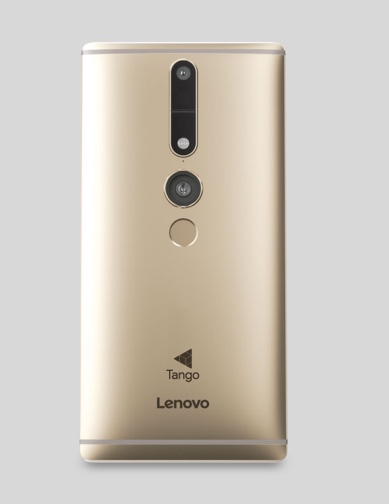
\includegraphics[height=4.5cm]{img/cap2/lenovo-phab2-pro.jpg}}
\hspace{0.5cm}
\subfigure[]{\label{fig:zenfone}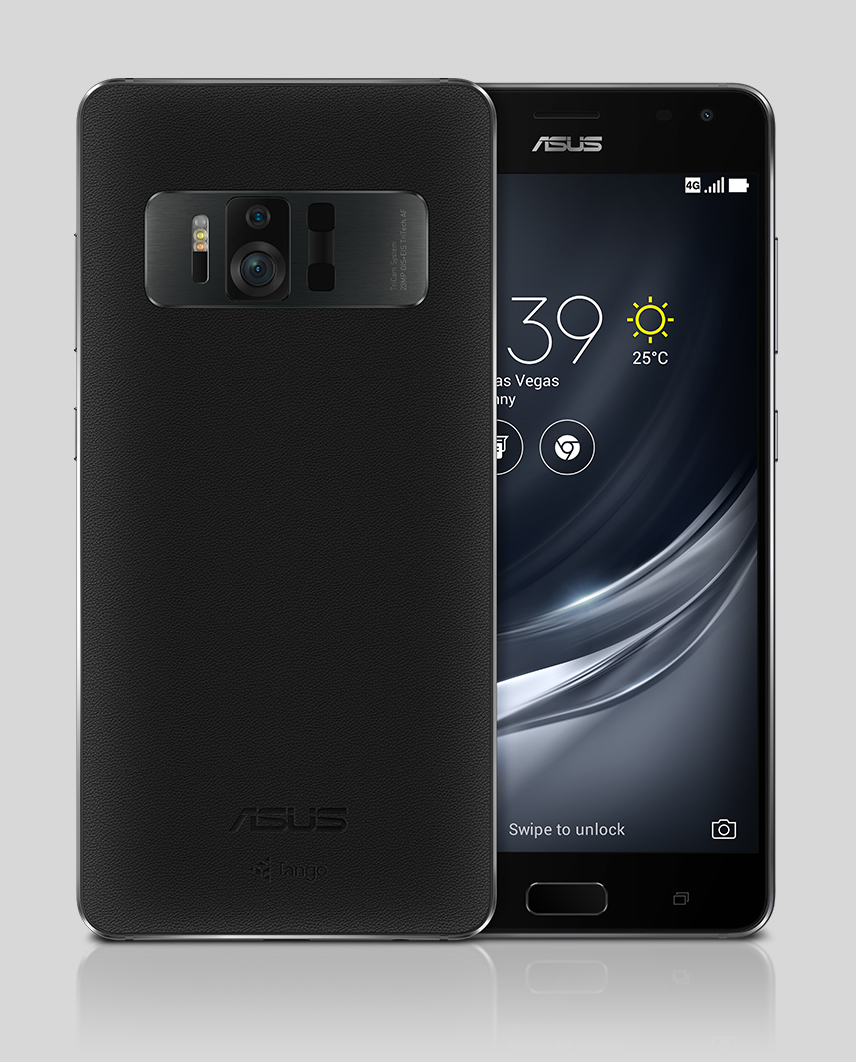
\includegraphics[height=4.5cm]{img/cap2/asus-zenfone-ar.jpg}}
\hspace{0.5cm}
\subfigure[]{\label{fig:prototipoTango}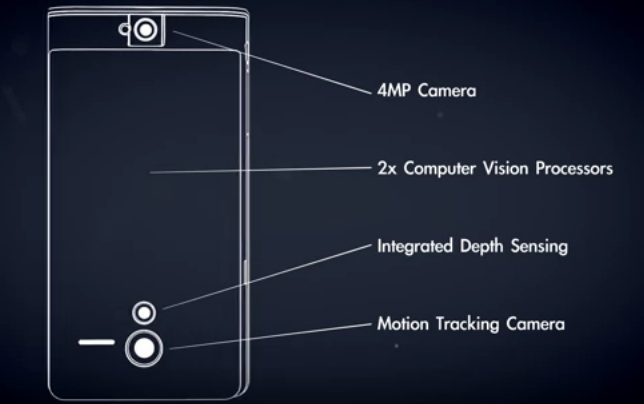
\includegraphics[height=4.5cm]{img/cap2/prototipo_Tango_smartPhone.png}}
\hspace{0.5cm}
\end{center}
\caption{El primer smartphone compatible con Tango de Lenovo(a). El primer Smartphone compatible con Tango y DayDream de ASUS (b).Esquema de prototipo de smartphone Tango (c).}
\end{figure}
Las posibilidades que ofrecerán este tipo de dispositivos serán muy variadas, desde medir las dimensiones de la habitación, hasta lo más útil como guiar a personas con discapacidades visuales en el interior de edificios. Pero también tendrá utilidades para el entretenimiento como convertir una habitación en el escenario de un juego mediante realidad aumentada.

Al ser una tecnología nueva aún no hay un elevado número de dispositivos que lo soporten. De momento existen 2 móviles compatibles con Tango \footnote{https://get.google.com/tango/}, el Lenovo  Phab 2 pro (Figura \ref{fig:lenovo}) y el Asus Zenfone AR (Figura \ref{fig:zenfone}).
En el caso del Zenfone AR  estará equipado con 3 cámaras traseras, una para seguir objetos (\textit{motion tracking}), otra para detectar profundidad y otra de alta resolución de 23 MP.
Con estas 3 cámaras el smartphone podrá crear una modelo tridimensional del entorno y seguir su movimiento. La cámara de localización permitirá al ZenFone conocer su posición 3D en todo momento mientras se mueve por el entorno. La cámara de profundidad está equipada con un proyector de Infrarrojos que le permite medir distancias hasta los objetos en el mundo real.

\begin{figure}[htbp]
\begin{center}
\subfigure[]{\label{fig:mapaTango}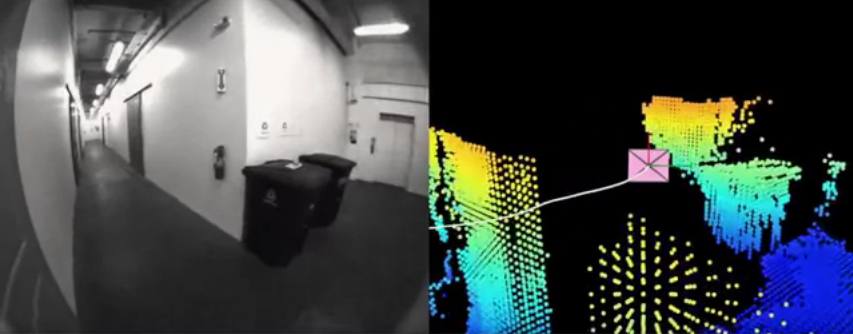
\includegraphics[height=3.0cm]{img/cap2/Proyecto_Tango_genera_mapa.png}}
\hspace{0.5cm}
\subfigure[]{\label{fig:makingMapTango}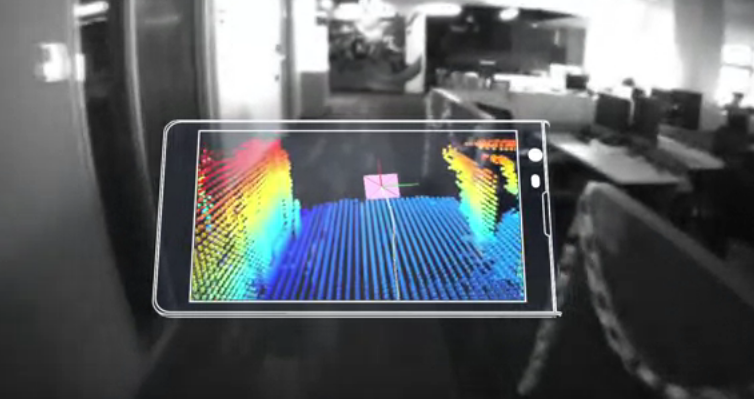
\includegraphics[height=3.0cm]{img/cap2/tangoDeviceMakingMap.png}}
\end{center}
\caption{Generación de mapa 1 (d). Generación de mapa 2 (e)}
\end{figure}

\clearpage

%\subsection{Magic Plan}
\item \textbf{Magic Plan:}

Magic Plan es una aplicación que permite de forma interactiva obtener planos de habitaciones o del interior de un edificio, utilizando para ello la cámara de nuestra tablet o smartphone, sólo es necesario sacar fotos. Esta aplicación es gratuita, aunque si se desea obtener el plano en formato digital (pdf, jpg, csv y otros) será necesario pagar una pequeña cantidad de dinero.
Es muy sencilla de utilizar y en cuestión de minutos se obtiene un plano fiable sin necesidad de medir, dibujar, mover muebles  y sin necesidad de ser un experto.
La aplicación utiliza técnicas de Visual SLAM y se apoya también en la información de los giroscopios de los dispositivos. Es compatible con Android y dispositivos Apple.

En el caso de Android, actualmente la última versión es compatible con el sistema Tango, por tanto el procedimiento de captura es mucho más sencillo, robusto y preciso  ya que  permite detectar con mayor exactitud todas las paredes de la habitación, visualizarlas en 3D y aplicar realidad aumentada.

%\begin{figure}[htbp]
%\begin{center}
%\subfigure[]{\label{fig:magicPlan}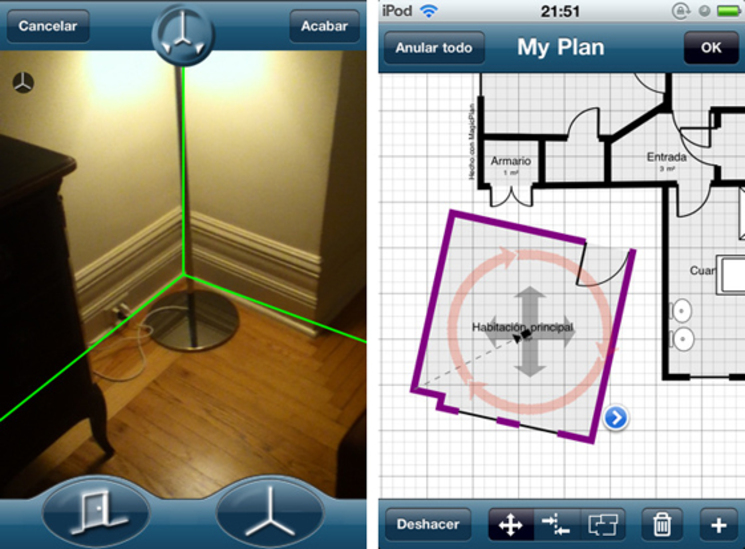
\includegraphics[height=8.0cm]{img/cap2/MagicPlan.jpg}}
%\end{center}
%\caption{La pantalla de un smartphone utilizando Magic Plan. }
%\end{figure}

%\clearpage

%\subsection{Pix4D}
\item \textbf{Pix4D:}

Pix4D \footnote{https://pix4d.com/} es un software especializado en fotogrametría. Permite la posibilidad de generar mapas 2D y 3D desde fotografías. Las imágenes pueden ser transmitidas vía wireless a Pix4DDim para procesarlas y convertirlas a mapas 2D y 3D.  Posteriormente esta información será accesible desde la nube para poder analizarlas y compartirlas.
Pix4D permite crear mapas con exactitud a partir de fotografías de interiores, también tiene aplicaciones en minería para medir superficies y volúmenes (Figura \ref{fig:volumen}) de minas a cielo abierto, incluso se utiliza con finalidades forenses para recrear en 3D escenarios de accidentes, que posteriormente pueden ser analizadas con todo detalle.
También tiene aplicaciones en la agricultura para obtener mapas de cosechas utilizando la información que proporcionan las cámaras especiales como la Parrot Sequoia (Figura \ref{fig:parrotSequoia}).
Con la aplicación Pix4DCapture podremos controlar un dron desde nuestro smartphone para que genere un mapa. El dron puede volar de forma autónoma siguiendo algunas de las trayectoria de vuelo que trae por defecto el producto o también puede generar el mapa mientras lo teledirigimos.

%\begin{figure}[htbp]
\begin{figure}[H]
\begin{center}
\subfigure[]{\label{fig:volumen}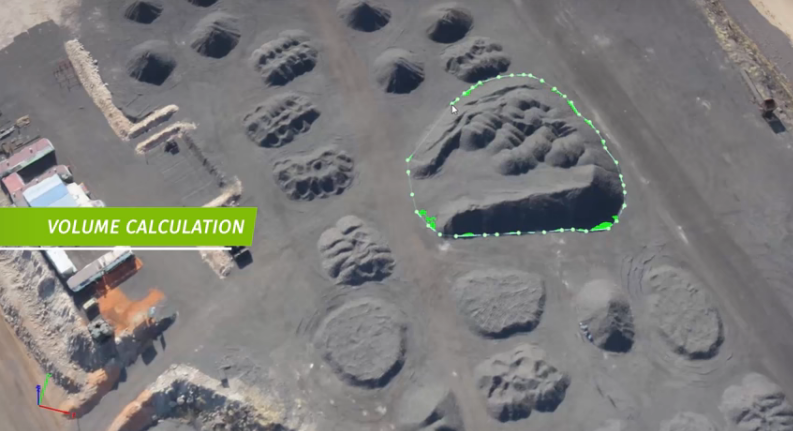
\includegraphics[height=3.0cm]{img/cap2/pix4d_volumen_calculo.png}}
%\hspace{0.5cm}
%\subfigure[]{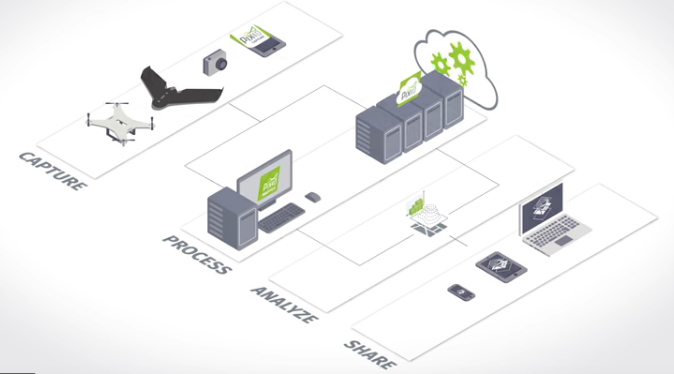
\includegraphics[height=3.0cm]{img/cap2/pix4d_esquema.png}}
%\hspace{0.5cm}
%\subfigure[]{\label{fig:dronTrayectoria}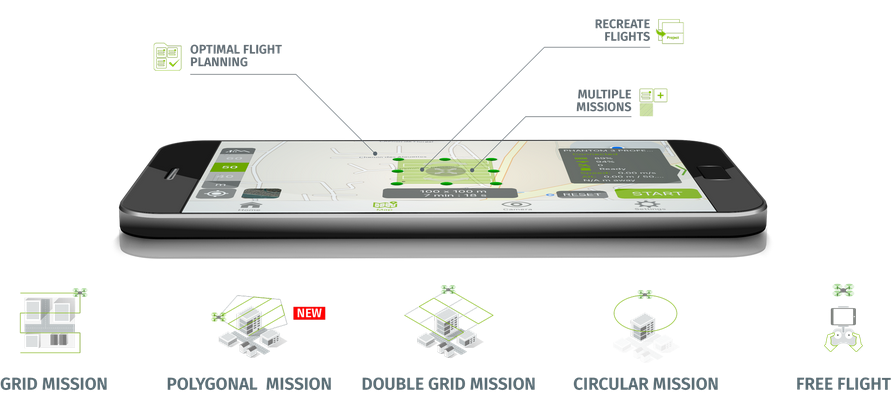
\includegraphics[height=4.0cm]{img/cap2/pix4d_dron_trayectorias.png}}
\hspace{0.5cm}
\subfigure[]{\label{fig:parrotSequoia}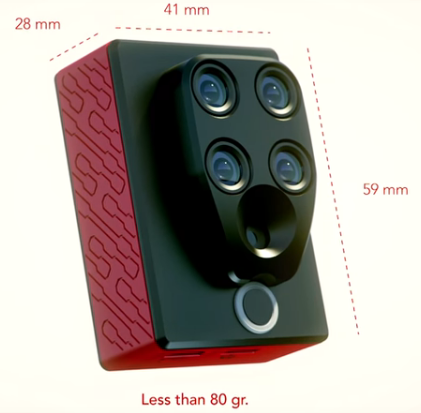
\includegraphics[height=4.0cm]{img/cap2/parrotSequoia.png}}
\end{center}
\caption{Pix4D cálculo de volumen(a). Cámara multiesprectral Parrot Sequoia (b)}
\end{figure}
%\clearpage

%\subsection{Photo Tourism}
\item \textbf{Photo Tourism:}

PhotoTourism o Photo Synth es un software inicialmente creado por la universidad de  Washington en colaboración con Microsoft. Es un sistema que toma grupos de conjuntos de fotografías disponibles online sobre un lugar en concreto, normalmente sobre un monumento turístico mundialmente conocido (como NotreDame, el Coliseo ( Figura \ref{fig:Coliseo}), La Fontana de Trevi) y es capaz de reconstruir puntos 3D de los monumentos y también calcular o estimar la posición de la cámara desde donde se tomaron las fotografías. Proporciona una nueva forma de navegar a través de fotografías de un destino turístico y una nueva forma de hacer visitas virtuales a monumentos.
Este sistema utiliza la técnica de \textit {Structure From Motion} SFM. SFM encuentra coincidencias de  puntos característicos entre distintas fotografías de un mismo lugar y que han sido tomadas desde distintos puntos de vista y así es capaz de calcular la localización 3D de dichos puntos característicos y también la localización 3D desde donde se tomaron las fotografías.
A diferencia de Visual SLAM, el procesamiento de estas fotografía es offline, sin necesidad de tiempo real, por lo que pueden ser ejecutadas desde un PC que por lo general tiene una capacidad de computación mucho mayor que una tablet o teléfono móvil.

\begin{figure}[htbp]
\begin{center}
\label{fig:Coliseo}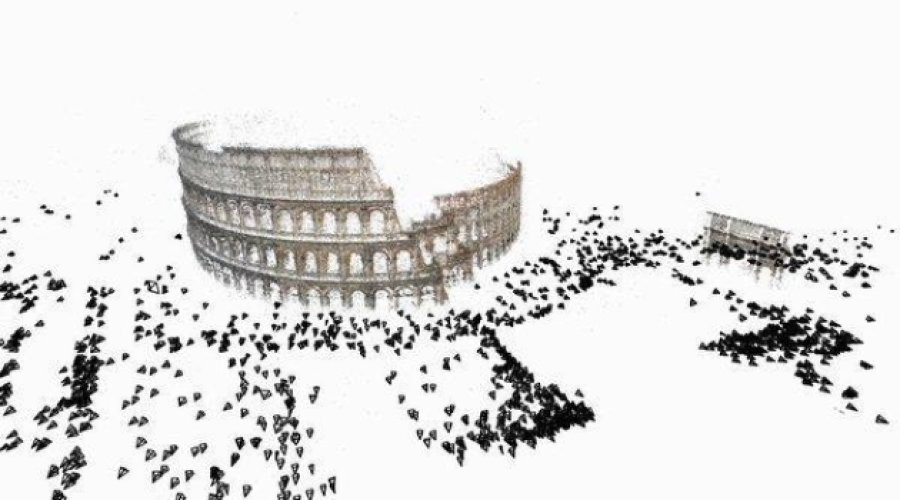
\includegraphics[height=8.0cm]{img/cap2/PhotoTourism.jpg}
\end{center}
\caption{Recreación del Coliseo de Roma generado con Photo Tourism. }
\end{figure}
%\clearpage

%\subsection{Canvas y el sensor Structure}


\item \textbf{Canvas y el sensor Structure:}

Canvas \footnote{https://canvas.io/ } es una herramienta de escaneo 3D enfocada a profesionales de la construcción o incluso aficionados al bricolaje en casa. La aplicación se ayuda del sensor de profundidad Structure. Este sensor se acopla en la parte trasera de un Ipad. Canvas permite obtener los planos en 3D de cualquier habitación de una manera fácil y sencilla, simplemente tendremos que pasear el Ipad equipado con el sensor Structure \footnote{https://structure.io/} alrededor de la habitación y podremos ver como el mapa 3D comienza a generarse en tiempo real. El sensor (Figura \ref{fig:Structure}) toma miles de medidas de profundidad que utilizará para generar el plano tridimensional. Los planos son almacenados en el Ipad y pueden ser consultados de manera interactiva posteriormente. Además permite que los planos generados sean convertidos a ficheros CAD.

\begin{figure}[htbp]
\begin{center}
\label{fig:Structure}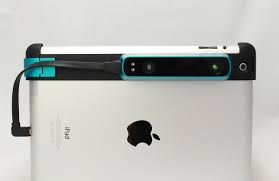
\includegraphics[height=5.0cm]{img/cap2/structureSensorCanvas.jpg}
\end{center}
\caption{El sensor de profundidad Structure para Ipad. }
\end{figure}

%\clearpage



\item \textbf{Robot Aspirador:}
Recientemente ha entrado en los hogares el uso de Visual SLAM gracias a los últimos modelos de aspiradora equipados con cámaras.
Estos aspiradores robotizados disponen de cámaras que le permiten obtener un mapa de la habitación o planta del edificio y gracias a este mapa son capaces de aspirar toda la superficie del suelo de la habitación de manera eficiente, sin dejar ninguna zona de la planta sin limpiar. Además están equipados con sensores de proximidad, que les permiten esquivar obstáculos y aunque tengan que modificar su recorrido momentáneamente son capaces de seguir limpiando ya que pueden utilizar el mapa para continuar su ruta. Entre los distintos aspiradores estarían:
Aspirador Dyson 360 Eye (Figura \ref{fig:Dyson})\footnote{http://www.dyson.come}, Aspirador Roomba 966 (Figura \ref{fig:roomba})\footnote{http://www.irobot.es/robots-domesticos/aspiracion}, Aspirador LG-Hombot \footnote{http://www.lg.com/es/aspiradoras/lg-VR64702LVMT}

Tanto el modelo de Dyson como Roomba utilizan una cámara de 360 grados, 
en cambio el modelo de LG utiliza una doble cámara, y es capaz de aspirar la casa incluso en la oscuridad.

%\begin{figure}[htbp]
\begin{figure}[H]
\begin{center}
\subfigure[]{\label{fig:Dyson}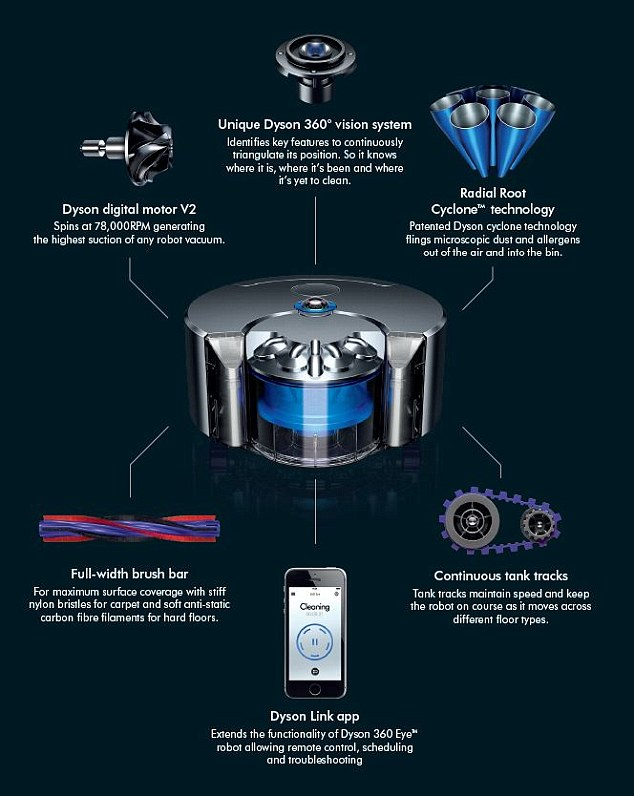
\includegraphics[height=6.0cm]{img/cap2/Dyson_360.jpg}}
\hspace{0.5cm}
\subfigure[]{\label{fig:roomba}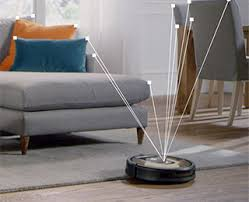
\includegraphics[height=6.0cm]{img/cap2/roomba_966.jpg}}
\hspace{0.5cm}
%\subfigure[]{\label{fig:LG_hombot}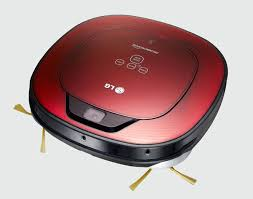
\includegraphics[height=6.0cm]{img/cap2/LG_hombot.jpg}}
\end{center}
%\caption{Robot Dyson 360 Eye (a) Robot Roomba 966 (b) Robot Hombot de LG (c).}
\caption{Robot Dyson 360 Eye (a) Robot Roomba 966 (b) }
\end{figure}

\item \textbf{Drones:}

Por último no podemos olvidar los drones, robots voladores equipados con cámara que también pueden obtener mapas de su entorno con Visual SLAM. Existen también proyectos para equipar a drones con dispositivos compatibles con Tango para que sean capaces de obtener mapas de interiores con mayor precisión, robustez y velocidad \footnote{http://spectrum.ieee.org/automaton/robotics/drones/autonomous-quadrotor-flight-based-on-google-project-tango}.


%\begin{figure}[htbp]
\begin{figure}[H]
\begin{center}
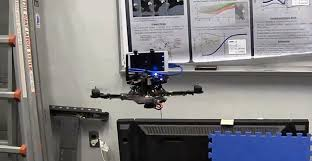
\includegraphics[height=5.0cm]{img/cap2/droneTango.jpg}
\end{center}
\caption{Dron equipado con dispositivo compatible con Tango}
\end{figure}

\end {enumerate}



\subsection{Conceptos}

Conviene explicar una serie de conceptos relacionados con Visual SLAM ya que aparecerán más adelante cuando expliquemos en profundidad los algoritmos más importantes que existen hoy en día para localización visual.

\textbf{Calidad}: La calidad del algoritmo de Visual SLAM dependerá de tres factores. La eficiencia temporal, la precisión espacial en la estimación de la posición y la robustez del algoritmo.

\textbf{Eficiencia}: Mediremos la eficiencia como el tiempo de ejecución de cada iteración del algoritmo. Los algoritmos deberán ser capaces de procesar al menos 30 fotogramas por segundo

\textbf{Precisión}:  El error lineal y error angular entre la posición estimada y la posición lineal determinará la precisión. Mediremos el error lineal como la distancia euclídea entre las dos posiciones, mientras que el error angular vendrá determinado por la diferencia entre las 2 orientaciones.

\textbf{Robustez}: Diremos que el algoritmo de localización es robusto siempre que pueda seguir funcionando con normalidad tras encontrarse con una situación imprevista (como una oclusión, secuestros, movimiento de objetos en la escena, mala calidad de imagen, etc)

\textbf{Oclusiones}: Cuando la cámara del robot esté tapada parcial o totalmente se producirá una oclusión, por tanto no se podrá extraer información en la región de la imagen ocluida. Los algoritmos deben estar preparados para cuando existan oclusiones.

\textbf{Secuestros}: Se producirá un secuestro cuando la cámara o robot sea movida deliberadamente por un tercero, de tal forma que los cálculos de la posición anterior ya no sean válidos. Los algoritmos deberían detectar secuestros e intentar localizarse desde su nueva posición.

\textbf{Localización Absoluta}: se produce cuando tenemos un mapa conocido, si estimamos la posición del robot dentro del mapa en coordenadas respecto del origen de coordenadas de ese mapa.

\textbf{Localización Incremental}:  En entornos con mapa desconocido, la localización del robot se establecerá de forma incremental respecto de posiciones previas pasadas ( por ejemplo en el instante anterior), lo que dará lugar a un error en la localización incremental que aumentará con el tiempo.

\textbf{Cierre de bucle}: Se produce cuando el robot vuelva a pasar por una zona del mundo que ya haya visitado anteriormente. Si se vuelve a pasar por el punto de origen se puede determinar el error que se ha producido comparando la posición real en el origen con la estimada por el algoritmo de localización.

\textbf{Relocalización}: Si tras un secuestro, el robot consigue recuperarse y estima correctamente la posición absoluta del robot dentro del mapa.


\subsection{Problemas abiertos en Visual SLAM} \label{s:problemavlsam}

Actualmente las técnicas de Visual SLAM presentan algunos problemas o inconvenientes que todavía son difíciles de sortear en la práctica. En esta sección presentaremos algunos de ellos:
\begin {enumerate}
\item \textbf{Inicialización del Mapa:}

Si en Visual SLAM queremos conseguir una estimación lo más exacta posible de la posición de la cámara es necesario contar con una buena inicialización del Mapa. Se debe contar con un sistema de coordenadas globales definido, y se tomarán puntos de referencia del entorno como puntos iniciales del mapa en el sistema global de coordenadas. Utilizando este método podemos inicializar Visual SLAM en un sistema de coordenadas global en la tierra. La transformación de estos puntos iniciales al sistema de referencia global se realizará mediante homografía.

Objetos de referencia como objetos 3D también se han utilizado para obtener un sistema global de coordenadas, posiciones iniciales de la cámara son estimadas gracias al seguimiento de objetos de referencia.
En Mono SLAM (cap 3,sec 1), por ejemplo, se utilizan al menos 4 puntos 3D (que se corresponden con las esquinas de un folio) como objetos de referencia.

\item \textbf{Ambigüedad en la escala:}

En algunas aplicaciones con Visual SLAM se necesita información de escala absoluta. Para obtener una referencia de escala absoluta se pueden utilizar zonas de la anatomía del usuario, como la cara, su mano o el propio cuerpo u otros objetos de tamaño conocido. En todos estos métodos se asume que entre personas la diferencia de tamaño es mínima para dichas partes del cuerpo. Se han dado otras aproximaciones como utilizar algunos de los sensores con los que ya están equipados la mayoría smartphones tales como acelerómetros, giroscopios y sensores magnéticos. Para eliminar el ruido de estos sensores se utiliza una técnica de filtro de dominio de frecuencia.


\item \textbf{Dificultad para operar en entornos con pocas texturas:}

Visual SLAM utiliza el emparejamiento de píxeles o puntos característicos entre varios \textit{frames} consecutivos. El emparejamiento suele fijarse en esquinas, bordes  o puntos distintivos que fácilmente podrán localizarse entre frames. Pero cuando en el entorno hay pocas texturas o presenta una alta monotonía de texturas,  el emparejamiento es difícil de realizar ya que un punto en un fotograma podría corresponder con N puntos en el siguiente fotograma y por tanto se dispararía el error de posición. Quizá este sea uno de los problemas más difíciles de solucionar con Visual SLAM
\cite{Takafumi17}.

\section{Estructura del documento}
El presente documento está dividido en 6 secciones y trata de describir este TFM, cuya temática  es la creación de una herramienta de evaluación de algoritmos de Visual SLAM. 
El primer capítulo es una introducción a la Visión Artificial y Visual SLAM, donde se explica en que consiste Visual SLAM, sus aplicaciones y cuales son las principales dificultades que debemos solventar a la hora de implementar un algoritmo de Visual SLAM. 
El capítulo 2 será una descripción detallada de los principales objetivos del TFM.
El capítulo 3 estará dedicado al Estado del Arte de los algoritmos Visual SLAM, y también se expondrán las herramientas más conocidas hoy en día para la evaluación de algoritmos Visual SLAM. 
En el capitulo 4 hablaremos de SLAMTestbed, una herramienta software creada precisamente en este TFM para evaluación de algoritmos Visual SLAM.
En el capítulo 5 se expondrán los distintos experimentos y tests realizados para evaluar la herramienta SLAMTestbed.
Y por último, el capitulo 6, donde se muestran las conclusiones del TFM.


\end {enumerate}
%\vfill
%\\raggedbottom 
%\parskip=1pt
%\vspace*{1in}
\flushbottom
\clearpage
\newpage
\pagebreak





